%!TEX root=./Emile.tex
\subsection{Staatsgenese als organisiertes Verbrechen: Charles Tilly}

\epigraph{
		``homo homini lupus.''}
	{
		\emph{Thomas Hobbes - 1651
	}

Bei genauerem Hinschauen erkennt man, dass das Kursthema voraussetzt, dass Demokratie überhaupt erstrebenswert ist.
Da kollektiv verbindliche Entscheidungen einer Demokratie inhärent sind, braucht man einen Staat, der diese unter Zwang durchsetzt.
Die Entstehung von Staaten ist das Thema Charles Tillys.
Staaten definiert er hierbei über die Kontrolle der physischen Gewalt über ein Volk auf einem zusammenhängenden Territorium:

	\begin{quote}
		``national states: relatively centralized, differentiated organizations the officials of which more or less successfully claim control over the chief concentrated means of violence within a population inhabiting a large, contiguous territory.'' \citep[170]{Tilly-1985-aa}
\end{quote}

\paragraph{Wie entsteht ein Staat?}
Nach Tillys Modell ist die Entwicklung eines Staates immer mit kriegerischen und gewaltvollen Handlungen verbunden.
Er geht sogar so weit zu behaupten, dass Gewalt notwendig für die Entwicklung eines Staates ist.
Der Ausgangspunkt für die Entwicklung eines Staates, ist die Monopolisierung von Gewalt und Macht: ``governments organize and, wherever possible, monopolize violence'' \citep[171]{Tilly-1985-aa}.
\citeauthor{Tilly-1985-aa} sagt, dass in der vor-staatlichen Zeit mehrere gewaltausübende Parteien konkurrieren.
Die Beziehungen derer untereinander unterliegen dem Sozialdarwinismus, da jede Partei gegen jede Krieg führt und diejenige besteht, die  siegreich aus dem Konflikt hervorgeht. Jede Person oder Gruppe versucht dabei, ökonomisch gesehen, positive Skalenerträge zu erzielen und sich so durch technische oder organisatorische Innovationen einen Vorteil über die anderen Parteien zu verschaffen, um sich gegen die anderen als der Stärkste innerhalb eines geografischen Bereiches durchzusetzen \citep[vgl.][173]{Tilly-1985-aa}.
Dieses Handeln ist entscheidend für die Entwicklung eines Staates, denn es zeigt, dass ein Staat nicht etwa infolge von friedlicher Zusammenarbeit der Menschen entsteht, sondern immer an Machtkämpfe, Ausbeutung und Krieg gebunden ist: ``war making likewise led to state making'' \citep[183]{Tilly-1985-aa}.

Positive Skalenerträge bedeuten, dass die Gesamtkosten für die Herstellung eines Produktes mit steigender  Anzahl an hergestellten Gütern sinken \autoref{fig:skalenertraege} (\autopageref{fig:skalenertraege}).

\begin{figure}[htbp]
	\begin{center}
	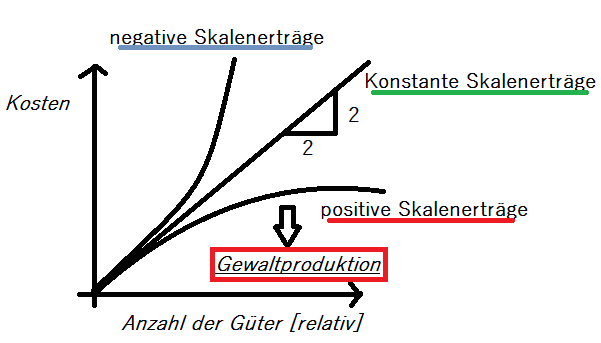
\includegraphics[width=1\textwidth]{img/Skalenertraege.png}
	\caption{Positive Skalenerträge}}
	\label{fig:skalenertraege}
	\end{center}
\end{figure}

Für die herrschende Partei ist das insofern ein Vorteil, dass sie mit geringeren Kosten effizienter Gewalt ``produzieren'' kann.
Positive Skalenerträge kommen vor allem durch technische und organisatorische Innovationen zustande.
So ist beispielsweise bei niedrig entwickelten Waffen wie Keulen kaum ein solcher Vorteil erkennbar, es kostet einen bestimmten Geldbetrag, eine Keule herzustellen, die  eine Person ausschalten kann, dieser Betrag bleibt aber auch bei den nächsten tausend produzierten Keulen ungefähr gleich, es ergibt sich dadurch kein großer Vorteil.
Anders bei höher entwickelten Waffen wie der Wasserstoffbombe.
Hat diese bei einem Ertrag von mehreren Millionen Menschen, die auf einmal ausgeschaltet werden können, bei der ersten Herstellung noch extrem große Produktionskosten, so werden diese bei den nächsten produzierten Bomben deutlich kleiner.
Für die herrschende Partei stellt dies einen militärischen Vorteil dar, er kann mit höherer Produktion deutlich höhere Erträge bei gleichen Kosten erzielen und so die Konkurrenten ausschalten.

Durch seine Macht hat die herrschende Partei nun die Möglichkeit, von seinem Volk  Tribute (Steuern) einzufordern und im Gegenzug \emph{Sicherheit} anzubieten.
Allerdings funktioniert dies nur durch die Gewaltpräsenz und somit die Bedrohung des Herrschers auf seine Untergebenen: ``governments are in the business of selling protection'' \citep[175]{Tilly-1985-aa}.
Der gebotene Schutz kann laut \citeauthor{Tilly-1985-aa} zwei Formen annehmen:

	\begin{enumerate}
		\item Verhält sich die herrschende Partei als \emph{legitimate protector} (legitimer Beschützer), so schützt sie das unterworfene Volk vor externen Angriffen.

		\item Ist der Machthaber ein \emph{racketeer} (Schutzgelderpresser), nutzt er sein Gewaltmonopol aus, indem er sein Volk unter Druck setzt.
	\end{enumerate}

\citeauthor{Tilly-1985-aa} betont dabei den paradox scheinenden Kontrast: der Staat droht mit Gewalt und schützt gleichzeitig vor ihr.

Wenn sich ein Staat wie ein Schutzgelderpresser verhält, also (hohe) Tribute fordert, das Geld aber nicht zum Wohle des Volkes nutzt sondern sich nur persönlich bereichert, spricht \citeauthor{Tilly-1985-aa} von Despotie.
Hätte das Volk aber als solches die Möglichkeit, Steuern zu regulieren und über ihre Verwendung zu entscheiden, läge eine Demokratie vor (\citep[vgl.][176]{Tilly-1985-aa}).
Krieg macht es dem Staat möglich, seine Macht nach außen zu expandieren und legitimiert innerhalb seines Einflussbereiches das Eintreiben von Steuern. Das Eintreiben von Steuern  wiederum macht es dem Staat möglich, Krieg nach außen zu führen. Durch diese wechselseitige Beziehung wird die Wirtschaft, besonders die Gewaltproduktion, angekurbelt.
Das intensiviert den Kreislauf zusätzlich.

\paragraph*{Durch welche Handlungen definiert sich ein Staat?}
Nachdem der Staat durch \emph{Unterwerfung} das Machtmonopol installiert hat (\citep[vgl.][175]{Tilly-1985-aa}), \emph{definiert} er sich durch das sogenannte \emph{Gewaltmonopol}: ``the authority's monopoly of force'' \citep[vgl.][172]{Tilly-1985-aa}.
In Tillys Verständnis kann man dies als das Alleinrecht auf Sicherheit und Ordnung auf einem bestimmten Gebiet verstehen: ``governments claim to provide protection'' \citep[vgl.][172]{Tilly-1985-aa}.
Andere Leistungen wie z.B. eine Krankenversicherung oder die Deutsche Schülerakademie sind nicht Teil von Tillys Staatsverständnis \citep[vgl.][181]{Tilly-1985-aa}.

% ## Gewaltmonopol und Schule
% Der Bezug zum eigentlichen Thema dieser Arbeit mag erst schleierhaft erscheinen.
% Doch \citeauthor{Tilly-1985-aa} begründet die Herkunft des Gewaltmonopols eines Staates, das auch die Basis für die Durchsetzung der Schulpflicht ist.
% Nach diesem Exkurs in die Staatstheorie handelt der nächste Text von gegenseitigem Helfen in der Schule.